\chapter{Controller Design for the TU/e \texorpdfstring{$1$}{1}-DoF System}
\label{chap:application}
In this chapter, the synthesis conditions of the previous chapter is applied to a $1$-DOF experimental setup. Different
uncertainty structures are considered and compared. 

\begin{figure}%
\centering
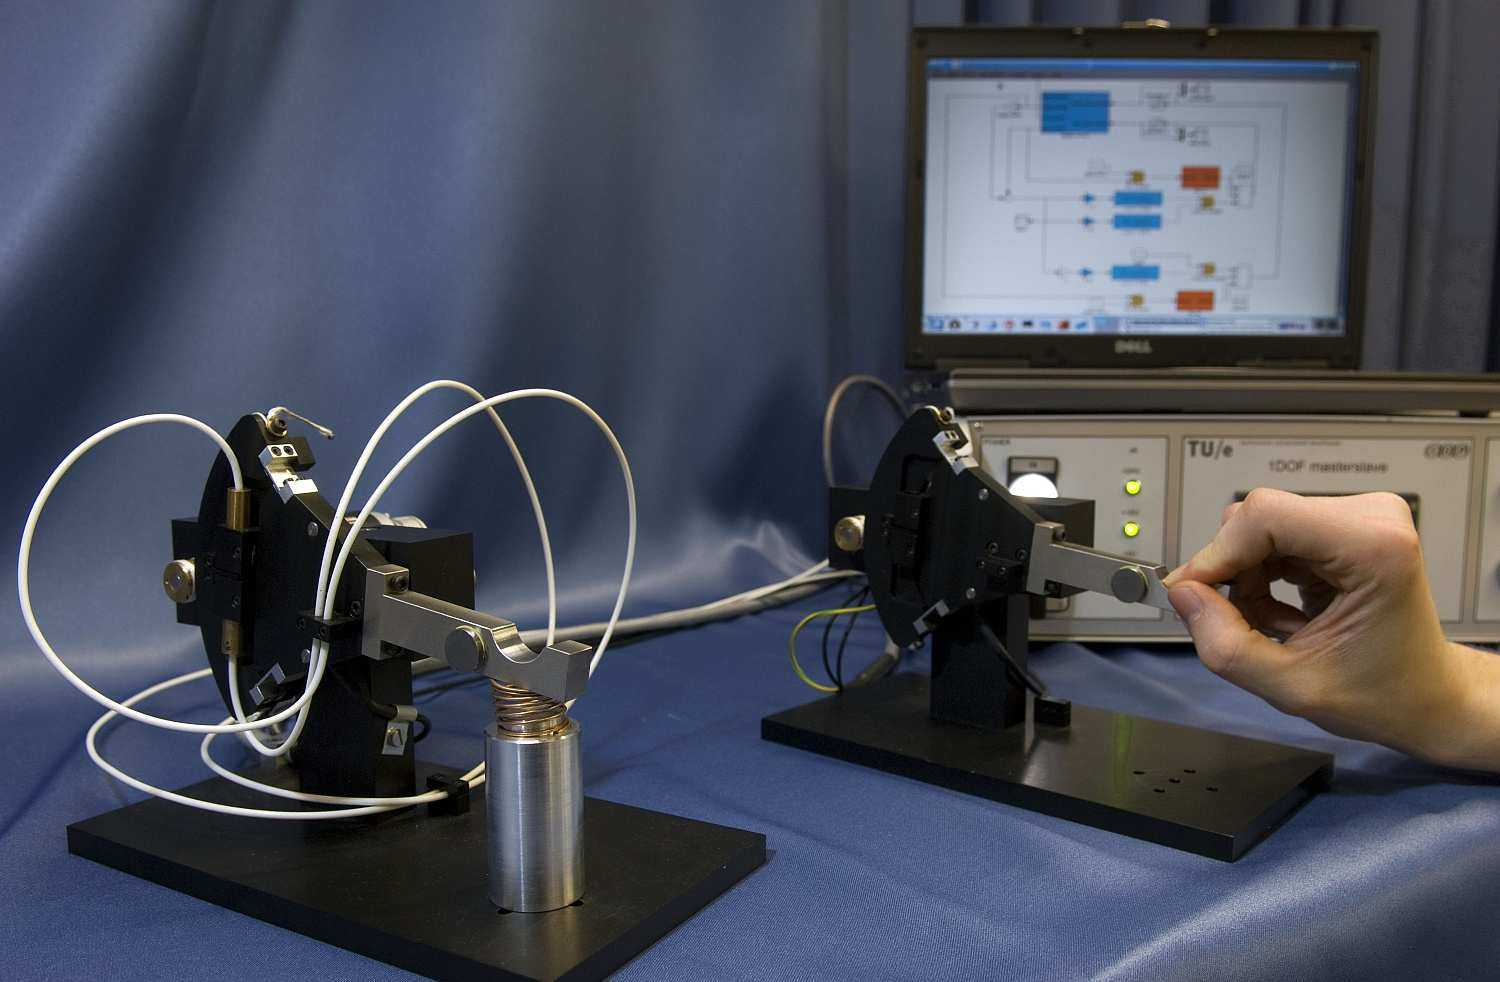
\includegraphics[width=0.6\columnwidth]{\impath/application/hendrix1dof}%
\caption[TU/e $1$-DoF Experimental Setup]{TU/e $1$-DoF Experimental Setup (Image is taken from \cite{hendrix})}%
\label{fig:app:onedof}%
\end{figure}

\section{The experimental setup}
At the Control Systems Technology department of Eindhoven University of Technology, a 1-Degree-of-Freedom prototype has been realized 
within the project of constructing a 5-DoF haptics local device for robotically assisted eye surgery(\cite{hendrix}). The setup is shown 
in \Cref{fig:app:onedof}. The actuation is provided to a capstan drive via a DC servo motor Maxon RE 35 which is connected to a statically 
balanced circular strip plate. This piece is also connected to an inner segment via elastic elements and the relative motion of these 
pieces make it possible to obtain a force measurement. An additional linear piece attached to the inner segment for handling the device. 
Due to the capstan mechanism, there is a rotational reduction of $i=\frac{1}{10}$. The system consists of four major inertial components; 
the motor and the encoder, outer strip segment, inner segment and the linear end-effector. The physical values are given in 
\Cref{tab:app:values}. The system can be approximated by the block diagram depicted in \Cref{fig:app:blodia}.
\begin{table}%
\caption{Physical Values of the Experimental Setup}
\centering
\begin{tabular}{l S l S l S}
\toprule
\multicolumn{2}{c}{Inertia \si{\kilo\gram\meter\squared}} &\multicolumn{2}{c}{Stiffness \si{\newton\meter\per\radian}}\\
\midrule
$J_{mot+enc}$   &7.0e-6  &$k_{mot}$   &1.5e2\\
$J_{pulley}$    &4.6e-7  &$k_{wire}$  &2.9e3\\
$J_{outer}$     &2.7e-4  &$k_{ts}$    &3.5e3\\
$J_{inner+end}$ &4.4e-4  &$k_{mot,b}$ &7.9e3\\
\bottomrule
\end{tabular}
\label{tab:app:values}
\end{table}




\begin{figure}[b]%
\centering
\begin{tikzpicture}[spring/.style={decoration={coil,pre length=#1,post length=#1,amplitude=1mm,segment length=1mm},decorate},
blodia/.style={draw,minimum height=1cm,minimum width=1.5cm},
scale=0.6,transform shape]
\coordinate (o) at (0,0);
\node[blodia] (pulley) at (-2cm,-2cm) {$J_{pulley}$};
\node[blodia,left= 2cm of pulley] (motenc) {$J_{mot+enc}$};
\node[blodia,anchor=west] (outer) at (4.0cm,1cm) {$J_{outer}$};
\node[blodia,right= 2cm of outer] (inner) {$J_{inner+ee}$};
\draw[spring=3mm] (motenc) -- (pulley)node[pos=0.5,above=3mm] {$k_{mot}$};
\draw (pulley) -| (o|-outer);
\draw[spring=3mm] (o|-outer) --++(2cm,0cm)node[pos=0.5,above=3mm] {$k_{mot,b}$} coordinate (temp);
\draw[spring=3mm] (temp) --(outer) node[pos=0.5,above=3mm] {$k_{wire}$};
\draw[spring=3mm] (outer) --(inner) node[pos=0.5,above=3mm] {$k_{ts}$};
\draw (o)--++(150:3mm)--++(-90:3mm) -- cycle;
\foreach\x in{-1,...,4}\draw[ultra thin] (150:3mm)++(0,-\x mm) --++(120:1.5mm);
\draw(150:3mm)++(0,2 mm) --++(0,-6.5mm);
\node (i) at (.6cm,0) {$i=\frac{1}{10}$};
\fill (o) circle (1.5pt);
\draw[-stealth] (motenc.west) |- ([yshift=5mm]motenc.north) node[above left] {$u(t)$};
\draw[-stealth] (motenc.west) |- ([yshift=-5mm]motenc.south) node[below left] {$\varphi(t)$};
\end{tikzpicture}
\caption[Simplified block diagram of the experimental setup ]{Simplified block diagram of the experimental setup (Adapted from \cite{
hendrix})}%
\label{fig:app:blodia}%
\end{figure}
If we enumerate all the blocks from left to right, starting from one to four, then the mathematical model of each device is given by:
\begin{align}
\frac{J_1}{i} \ddot{x}_1           &= \frac{u}{i} - \frac{k_1}{i}(x_1 - x_2)\\
\frac{J_2}{i} \ddot{x}_2 &= \frac{k_1}{i}(x_1 - x_2)-k_c(ix_2-x_3)\\
J_3 \ddot{x}_3           &= k_c(ix_2-x_3) - k_4(x_3-x_4)\\
J_4 \ddot{x}_4           &= k_4(x_3-x_4)
\end{align}
where $k_c = \inv{(\frac{1}{k_{wire}}+\frac{1}{k_{mot,b}})}$ and $u$ is the motor input. The system response is shown in 
\Cref{fig:app:modfrf}. The identification and the model verification is also provided in \cite{hendrix}. Based on the 
frequency response data, we have also added damping to the model artificially both to improve the numerical properties 
of the model and also match the physical setup. The damping coefficients to each spring element/group is given in \Cref{%
tab:app:damp}. We will use the same model for the remote device in what follows below. 
\begin{table}%
\caption{The additional damping coefficients that are included in the model.}
\centering
\begin{tabular}{l S}
\toprule
\multicolumn{2}{c}{Damping \si[per-mode=fraction]{\newton\meter\per\radian\second}}\\
\midrule
$b_{mot}$   & 1.8e-3\\
$b_{wire+mot,b}$  & 1.0e-5\\
$b_{ts}$    & 1.0e-3\\
\bottomrule
\end{tabular}
\label{tab:app:damp}
\end{table}



\begin{figure}[b]%
\centering
\begin{tikzpicture}
	\begin{loglogaxis}[
	enlargelimits=false,
	grid=both,
	width=0.8\textwidth,height=5cm,
	ymin=5e-6,
	yticklabel={\pgfmathprintnumber[fixed]{\tick}},
	xlabel= Frequency,
	ylabel= Magnitude,
	x unit=\si{\hertz},
	y unit=\si{\decibel},
	log basis y=10,
  yticklabel={\pgfmathparse{20*(\tick)}\pgfmathprintnumber[fixed]{\pgfmathresult}},
	]
		\addplot[red,thick] table[x=freq,y=resp1] {plotdata/figappmodfrf.txt};
		\addplot[blue,dashed] table[x=freq,y=resp2] {plotdata/figappmodfrf.txt};
		\addlegendentry[font=\tiny,align=left,anchor=west]{Motor $\rightarrow$ Encoder}
		\addlegendentry[font=\tiny,align=left,anchor=west]{Motor $\rightarrow$ End Effector}
	\end{loglogaxis}
\end{tikzpicture}
\caption{The frequency response of the hypothetical models from the motor actuation to the position measurements.}%
\label{fig:app:modfrf}%
\end{figure}

Note that up to the first zero of the system, same behavior can be represented with a second order transfer
function 
\[
\tilde{G}(s) = \frac{1}{0.0015s^2 + 0.00287s + 0.25}.
\]
This simplification is used in \cite{cesarACC,cesarSYROCO} and the resulting controllers which are based on this model are 
experimentally implemented. Due to the low-frequency nature of the task, this simplification did not cause any problems 
during the experiments.

We nevertheless present the full model LFT interconnection structure but in the controller design cases only the simplified 
model is used. This is due to the fact that the system is altered significantly (e.g., the steel cables are replaced by plastic 
and the housing of the shafts are not in the optimal condition etc.) from its original construction. Hence, we have
used a simple model obtained from identification experiments.



\subsection{Incorporating the human dynamics}
To be able to model both cases of \enquote{user holding/released the device} and \enquote{remote device is in free-air/contact} 
cases we need to introduce a model of the possible human users and environment dynamics. However, those models are dependent on
grasp configuration, task-environment and other parameters. One can start with a predefined task case, say a MIS or a peg-in-hole 
assembly and limit the relevant cases that can occur together with some engineering safety tolerance. That would reduce the 
set of possible physically relevant operators significantly. In the absence of refined human and environment models, we would simply
follow the ubiquitous mass-spring-damper modeling paradigm as shown in \Cref{fig:app:attachhuman}. Here, we adopt the usage of an
external force model but this does not bring in any complications since we do not invoke any passivity assumptions. Moreover
we will assume that the parameters of the human dynamics are time-varying operators together with the low-pass filtered $f_h$ to 
emphasize the $\approx \SI{10}{\hertz}$ bandwidth. There is no structural distinction of applied force and human arm but we only 
model the relevant arm/hand trajectories thus the resulting combined response is not modified. Note that by adding another 
under-damped mass-spring-damper component to the human dynamics one can also model the hand tremor and motor noise if needed. 


\begin{figure}%
\centering
\begin{tikzpicture}[spring/.style={decoration={coil,pre length=#1,post length=#1,
amplitude=1mm,segment length=1mm},decorate},
blodia/.style={draw,minimum height=1cm,minimum width=1.5cm},
damper/.style={decoration={markings,  
  mark connection node=dmp,
  mark=at position 0.5 with 
  {\node (dmp) [inner sep=0pt,transform shape,rotate=-90,minimum width=5pt,minimum height=1pt,draw=none] {};
   \draw ([xshift=1pt]dmp.north east) -- (dmp.south east) -- (dmp.south west) -- ([xshift=1pt]dmp.north west);
   \draw ([yshift=-2pt]dmp.north) -- ([yshift=2pt]dmp.north);}}, decorate},
ground/.style={fill,pattern=north east lines,draw=none,minimum width=3mm,minimum height=10mm},
scale=0.8,transform shape]
\coordinate (outer) at (0,0);
\node[blodia,right= 2cm of outer] (inner) {$J_{inner+ee}$};
\draw[spring=3mm] ([yshift=2mm]outer) -- ([yshift=2mm]inner.west) node[pos=0.5,above=3mm] {$k_{ts}$};
\draw[damper] ([yshift=-2mm]outer) -- ([yshift=-2mm]inner.west) node[pos=0.5,below=2mm] {$b_{ts}$};
\draw[dashed] ([shift={(-5mm,-5mm)}]outer) -| (outer) |- ([shift={(-5mm,5mm)}]outer);
\node[draw,anchor=south east,minimum size=1cm] at (inner.north east) (humass){$m_h$};
\draw[spring=3mm] ([yshift=2mm]humass.east) -- ++(2cm,0mm)  node[pos=0.5,above=3mm] {$k_{h}$};
\draw[damper] ([yshift=-2mm]humass.east) -- ++(2cm,0mm) node[pos=0.5,below=2mm] {$b_h$};
\draw coordinate (t2) at ([xshift=2cm]humass.north east) (t2) -- (t2|-humass.south east);
\node[ground,anchor=north west] at (t2) {};
\draw[stealth-] (inner.-10) --++(1cm,0) node[below]{$F_h$};
\end{tikzpicture}
\caption[Including the uncertain human model in the system ]{Including the uncertain human model in the
 system shown in \Cref{fig:app:blodia}.}%
\label{fig:app:attachhuman}%
\end{figure}


The human arm model is identified experimentally for different grasp configurations (see, e.g., \cite{cesarSYROCO}). Then,
using these frequency response data, uncertainty intervals in which the parameters of the human arm varies through time are 
selected. The updated parameter intervals are given in \Cref{tab:app:humparam}\footnote{We keep using $m_h$ notation for 
convenience however it should be understood as $J_h$.}.

\begin{table}%
\caption[Identified Uncertain Human Parameters as Rotational Mechanical Components]{Identified Uncertain Human Parameters 
as Rotational Mechanical Components}
\centering
\begin{tabular}{r l l}\toprule
\multicolumn{3}{c}{Parameter Variation Intervals}\\\midrule
$m_h$ & $[0,0.53]$ &\si{\kilo\gram\meter\squared\per\radian}\\
$b_h$ & $[0,8.58]$ &\si{\newton\meter\second\per\radian}\\
$k_h$ & $[0,994.2]$ &\si{\newton\meter\per\radian}\\
$k_e$ & $[0,3000]$ &\si{\newton\meter\per\radian}\\
\bottomrule
\end{tabular}
\label{tab:app:humparam}
\end{table}

Next, we obtain the LFT interconnection of the uncertain model. We first write down the equations of motion of the combined inertial element $J_{inner+ee}$/$m_h$
\[
(J_4+m_h)\ddot{x}_4 = k_3(x_3-x_4) + b_3(\dot{x}_3-\dot{x}_4) - k_hx_4 - b_h\dot{x}_4 -f_h
\]
and hence
\[%\begin{align*}
\ddot{x}_4 = \inv{(J_4 + m_h)}\left(k_3(x_3-x_4) + b_3(\dot{x}_3-\dot{x}_4) - k_hx_4 - b_h\dot{x}_4 -f_h\right)
\]\[
           = {%\underbracket
                            \left(\frac{1}{J_4} - \frac{1}{J_4}\frac{m_h}{J_4}\inv{\left(1+\frac{m_h}{J_4}\right)}\right)%
                            }%
        \left(k_3(x_3-x_4) + b_3(\dot{x}_3-\dot{x}_4) - k_hx_4 - b_h\dot{x}_4 -f_h\right).
\]%\end{align*}
The first term in the second equality can be shown to be 
\[
\delta_{m_h}{\displaystyle\star}\pmatr{-\frac{m_h}{2J_4}&\frac{m_h}{2J_4}\\-\frac{1}{J_4}&\frac{1}{J_4}}
\]
with $\delta_{m_h}(t)\in[0,2]$ for all $t>0$. Then, labeling the remaining uncertain terms with uncertainty outputs we have
\begin{align}
\ddot{x}_4 &= \frac{1}{J_4}\bigg(k_3(x_3-x_4) + b_3(\dot{x}_3-\dot{x}_4) - \frac{m_h}{2J_4}p_1 - p_2 - p_3 -f_h\bigg)\\
p_1 &= \delta_{m_h}q_1\\
p_2 &= \delta_{b_h}q_2\\
p_3 &= \delta_{k_h}q_3\\
q_1 &= \bigg(k_3(x_3-x_4) + b_3(\dot{x}_3-\dot{x}_4) - \frac{m_h}{2J_4}p_1 - p_2 - p_3 -f_h\bigg)\\
q_2 &= \frac{b_h}{2}\dot{x}_4\\
q_3 &= \frac{k_h}{2}x_4
\end{align}
where $\delta_{m_h},\delta_{b_h},\delta_{k_h}\in[0,2]$ for all $t>0$. The resulting state equations are obtained as
\begin{alignat}{4}\label{eq:prestateequations1}
\hat{E}\dot{x} &= \hat Ax   &&+ \hat B_p p   &&+ \hat B_w w   &&+ \hat B_u u\\\label{eq:prestateequations2}
q        &= \hat C_qx &&+ \hat D_{pq}p &&+ \hat D_{wq}w &&+ \hat D_{uq}u
\end{alignat}
where 
\begin{equation}
\hat E =\pmatr{
\multirow{4}{*}{\scalebox{1.5}{$I_4$}} &   &             &   &   \\
                                       &   &             &   &   \\
                                       &   &             &   &   \\
                                       &   &             &   &   \\                                                        
                                       &J_1&             &   &   \\
                                       &   &\frac{J_2}{i}&   &   \\
                                       &   &             &J_3&   \\
                                       &   &             &   &J_4
},
\hat B_p = 
\pmatr{
0   &0   &0   \\
0   &0   &0   \\
0   &0   &0   \\
0   &0   &0   \\
0   &0   &0   \\
0   &0   &0   \\
0   &0   &0   \\
-\frac{m_h}{2J_4}   &-1   &-1
},
\hat B_w = 
\pmatr{0\\0\\0\\0\\0\\0\\0\\-1},
\hat B_u = \pmatr{0\\0\\0\\0\\1\\0\\0\\0}
\label{eq:eqrotmodelE}
\end{equation}

\begin{equation}
\hat A = \pmatr{
\multicolumn{4}{c}{\multirow{4}{*}{\scalebox{1.5}{$0_4$}}} &\multicolumn{4}{c}{\multirow{4}{*}{\scalebox{1.5}{$I_4$}}}\\
&&&&&&&\\
&&&&&&&\\
&&&&&&&\\
-k_1          &k_1                 &0        &0    &-b_1          &b_1                   &0         &0   \\
\frac{k_1}{i} &\frac{-k_1}{i}-ik_2 &k_2      &0    &\frac{b_2}{i} &\frac{-b_2}{i}-ib_2   &b_2       &0   \\
0             &ik_2                &-k_2-k_3 &k_3  &0             &ib_2                  &-b_2-b_3  &b_3 \\
0             &0                   &k_3      &-k_3 &0             &0                     &b_3       &-b_3
}
\label{eq:rotmodelA}
\end{equation}
\begin{multline}
\hat Cq = \pmatr{
0 &0 &k_3 &-k_3 &0 &0 &b_3 &-b_3\\
0 &0 &0   &0    &0 &0 &0   &\frac{b_h}{2}\\
0 &0 &0   &\frac{k_h}{2}    &0 &0 &0   &0
},\\ 
\hat D_{pq} = \pmatr{\frac{m_h}{2J_4} &-1 &-1\\0&0&0\\0&0&0},
\hat D_{wq} = \pmatr{-1\\0\\0}, 
\hat D_{uq} = \pmatr{0\\0\\0},
\label{eq:rotmodelCq}
\end{multline}
The position measurements are done at the 
motor location with an encoder and the force measurements are based on the relative motion of the $J_{inner+ee}$ and
$J_{outer}$ since the elasticity of the coupling is known. This leads to the following measurement channel structure:
\begin{multline}
\hat Cy = \pmatr{
1 &0 &0   &0    &0 &0 &0 &0\\
0 &0 &k_3 &-k_3 &0 &0 &0 &0\\
},\\ 
\hat D_{py} = \pmatr{0 &0 &0\\0&0&0},
\hat D_{wy} = \pmatr{0\\0\\0}, 
\hat D_{uy} = \pmatr{0\\0\\0},
\label{eq:rotmodelCy}
\end{multline}

\subsection{Incorporating the environment dynamics}
The remote device is simply another copy of the local device, hence shares the same structure given by
\eqref{eq:prestateequations1},\eqref{eq:prestateequations2}. For the remote device, we only consider a spring with time-varying characteristics however it can also be assumed to admit 
a more detailed structure similar to the human dynamics. It's relatively simpler to obtain the LFT interconnection since we 
can simply remove the $\delta_{m_e},\delta_{b_e}$ uncertainty channels such that only the environment stiffness coefficient
remains uncertain. We will assume that the environment stiffness can change arbitrarily fast in order to model hard contacts
or sudden release from a constraint, say, sliding over an edge. The uncertainty matrices are modified such that
\[
q = k_e x_4, p = \delta_{k_e} q.
\]
The environment uncertainty is selected as a time-varying parameter $k_e\in[0,3000]$ \si{\newton\meter\per\radian} to model 
the relatively high stiff contacts.


\subsection{The Generalized Plant Model}
Combining the both device models, we can then define the performance channels. For the force tracking we select the error of 
the force measurements to be minimized. For the position tracking we select the devices' encoder reading difference to be 
minimized. We also penalize the actuator outouts to make the numerical optimization problem healthier. We will further emphasize 
the frequency bands of interest with frequency dependent weights defined below. Translating these into 
the matrix form, we obtain the following plant $G\in\mathcal{RH}_\infty^{(n_q+n_z+n_y)\times(m_p+m_w+m_u)}$
\begin{equation}
%\pmatr{\dot{x}\\\hline q\\ z\\ y} = 
G \coloneqq \left[
\begin{array}{c|ccc}
	A    &B_p    &B_w    &B_u\\\hline
	C_q  &D_{pq} &D_{wq} &D_{uq}\\
	C_z  &D_{pz} &D_{wz} &D_{uz}\\
	C_y  &D_{py} &D_{wy} &0
\end{array}
\right]
%\pmatr{x\\ p\\ w\\ u}
\label{eq:app:genplantsymb}
\end{equation}
with particular entries are defined as the following; let $e_\frac{i}{8}$ denote the 
$i$\textsuperscript{th} column of the $8\times 8$ identity matrix,
\[
\begin{array}{rl}
A      &= I_2\otimes\hat{A}  \\
B_p    &= \pmatr{\hat{B}_p&0\\0&-e_{\frac{8}{8}}}\\
B_w    &= I_2\otimes\hat{B}_w\\
B_u    &= I_2\otimes\hat{B}_u\\
C_y    &= I_2\otimes\hat{C}_y\\
D_{py} &= 0\\%I_2\otimes\hat{D}_{py}\\
D_{wy} &= 0\\%I_2\otimes\hat{D}_{wy}\\
C_q    &=\pmatr{\hat{C}_q &0\\0&\displaystyle\frac{k_e}{2}e^T_\frac{4}{8}}\\
D_{pq} &= \pmatr{\hat{D}_{pq} &0\\0&0}\\
D_{wq} &= \pmatr{\hat{D}_{wq} &0\\0&0}\\
D_{uq} &= 0\\%\pmatr{\hat{D}_{uq} &0\\0&0}
\end{array}
\]
Then, the performance channels are given by
\[
\begin{array}{rl}
z = \pmatr{x_l-x_r\\f_l-f_r\\u_l\\u_r}
\end{array}
\]
\[
C_z = \pmatr{e_\frac{1}{8}^T &-e_\frac{1}{8}^T\\k_3(e_\frac{3}{8} -e_\frac{4}{8})^T &-k_3(e_\frac{3}{8} -e_\frac{4}{8})^T\\ \multicolumn{2}{c}{0}\\ \multicolumn{2}{c}{0}}
\]
\[
D_{py} = 0, D_{wy} = 0
\]
Thus, we have obtained a plant-uncertainty interconnection $\Delta-G$ where 
\begin{equation}
\Delta\coloneqq \pmatr{\delta_{m_h}&&&\\&\delta_{b_h}&&\\&&\delta_{k_h}&\\&&&\delta_{k_e}}
\label{eq:realisticunc}
\end{equation}


%\subsection{Input/Output Weights Selection}
%Once we obtain the generalized plant, the performance channels are weighted to emphasize the frequency band of 
%interest.
%
%\subsubsection{Input Weight}
%The human force is modeled as an external input to the system and without a weight it is only assumed to be a 
%finite energy signal with no additional constraints. However, we are aware of the fact that the frequency 
%spectrum of the human input is negligible beyond \SI{\approx 10}{\hertz}. Similarly the environment force spectrum
%is also not relevant since the environment uncertainty models the spring action up to \SI{3000}{\newton\meter\per\radian}.
%Thus, both channels are prefiltered with low-pass filters to constrain the possible inputs.
%%
%\[
%W_f = \frac{20\pi}{s+20\pi}
%\]
%
%
%\subsubsection{Output Weights}
%The position tracking error spectrum is nominally limited to the external inputs to the system since the position change
%is due to the human and environment forces acting on the system. For an additional safety factor, we choose the bandwidth
%of the filter to be around \SI{100}{\hertz}. 
%%
%\[
%W_{pos} = \frac{2\cdot10^4\pi}{s^2 + 180\pi s+2\cdot10^4}
%\]
%



\subsection{Simplified System Model}
In the previous publications, \cite{cesarACC,cesarSYROCO} the simplified model is utilized while capturing the essential 
complications making the problem substantially simpler. We have followed the same idea by adopting the scheme depicted in 
\Cref{fig:app:simpdiag}. In this simplified model, the dynamics of the devices are lumped into second-order mass-spring-damper 
models and the human/environment dynamics are interconnected directly to the corresponding device models. 

\begin{figure}
\centering
\begin{subfigure}{0.4\linewidth}
\centering
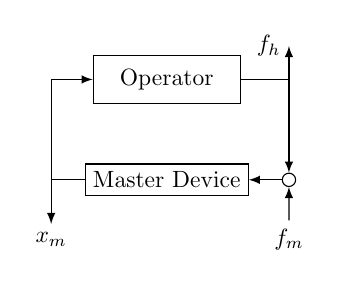
\begin{tikzpicture}[>=latex,scale=0.85,transform shape]
\node[draw,inner xsep=4mm,inner ysep=2mm] (op) at (0,1.5) {Operator};
\node[draw] (mas) at (0,0) {Master Device};
\node[circle,draw,inner sep=2pt] (sum) at ([xshift=6mm]mas.east) {};
\draw[->] (op) -| (sum);
\draw[<-] (mas) -- (sum);
\draw[->] ([yshift=-5mm]sum.south) node[below](fm){$f_m$}-- (sum);
\draw[->] (op-|sum) -- ++(0,5mm)node[left] {$f_h$};
\draw[->] (mas.west) -| ++(-5mm,5mm) |- (op);
\node (xm) at ([xshift=-5mm]mas.west|-fm) {$x_m$};
\draw[->] (mas) -|(xm);
\end{tikzpicture}
\caption{}
\label{fig:app:simpdiaga}
\end{subfigure}
\hfill
\begin{subfigure}{0.4\linewidth}
\centering
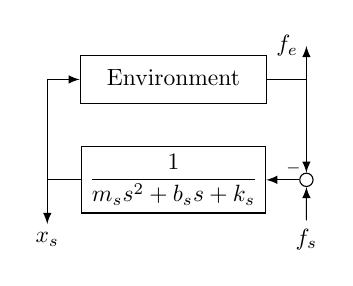
\begin{tikzpicture}[>=latex,scale=0.85,transform shape]
\node[draw,inner xsep=4mm,inner ysep=2mm] (op) at (0,1.5) {Environment\vphantom{p}};
\node[draw] (mas) at (0,0) {$\displaystyle \frac{1}{m_ss^2+b_ss+k_s}$};
\node[circle,draw,inner sep=2pt] (sum) at ([xshift=6mm]mas.east) {};
\draw[->] (op) -| (sum);
\draw[<-] (mas) -- (sum);
\draw[->] ([yshift=-5mm]sum.south) node[below](fm){$f_s$}-- (sum);
\draw[->] (op-|sum) -- ++(0,5mm)node[left] {$f_e$};
\draw[->] (mas.west) -| ++(-5mm,5mm) |- (op);
\node (xm) at ([xshift=-5mm]mas.west|-fm) {$x_s$};
\draw[->] (mas) -|(xm);
\node (min) at ([shift={(-1mm,1.2mm)}]sum.150) {$\scriptstyle -$};
\end{tikzpicture}
\caption{}
\label{fig:app:simpdiagb}
\end{subfigure}
\caption{Diagram of (a) operator/master device and (b) environment/slave device.}
\label{fig:app:simpdiag}
\end{figure}

For the performance objectives, it has been selected to minimize the position error $x_m-x_s$ and 
the force error $f_h-f_e$, as opposed to minimizing $f_h-f_s$ and $f_e-f_m$ independently. In other words
it is the interaction forces we desire to match but not the individual force reference signals at each side. 
However, this has an inherent well-posedness problem when the user releases the device. As can be seen in 
\Cref{fig:app:design1}, when the user dynamics are absent there is no control authority left to influence 
$f_h$ (and $f_e$ too due to the same reasoning). Therefore, the system (control design problem) is analytically 
uncontrollable (infeasible) for the full uncertainty region. However this can be avoided by allowing for 
slight tolerances to account for the modeling imperfections and to avoid this analytical pathology. 

The reason for this artificial problem is the over-simplification of the model since in the original model 
the force sensor is not collocated with the human input. The force measurements are in fact obtained 
via the relative motion of the outer and inner segments as we have modeled above. However, before we discard 
this modeling approach, we would like to emphasize that the device is not ideally free from any friction and 
measurement uncertainties. Thus even untouched the model still involves joint and cable frictions and unmodeled
inertial asymmetries which can be lumped into the human dynamics. Therefore, all these hard-to-model effects 
can be reflected to the already uncertain human model. As a practical example, the friction of the device can 
be attributed to the damping uncertainty of the human model. Hence, one can always assume that a minimal 
interaction with the human is always present even though this minimal interaction might be due to the angular 
inertia, friction etc. 

In the sequel, we will design three controllers with different uncertainty class assumptions. The first two 
cases will be using fixed mass and damping coefficients depicted in \Cref{fig:app:design1}. 

\section{Three Controller Design Cases}



\begin{figure}%
\begin{subfigure}[b]{.45\linewidth}
\centering
\begin{tikzpicture}[>=latex,mygain/.style={isosceles triangle,draw,
shape border rotate=180,
isosceles triangle apex angle=60,
inner sep=0,minimum height=7mm},myinteg/.style={draw,minimum height=9mm},
sum/.style={circle,draw,inner sep=2pt},scale=0.87,transform shape,mygainrev/.style={mygain,mygain,shape border rotate=0},
scale=0.75]
\draw[dotted] (-0.5cm,-0.5cm) rectangle (7.5cm,2.6cm);
\draw[dotted] (-0.5cm,5.5cm) rectangle (7.5cm,2.8cm);
\node[myinteg] (integ1) at (1cm,2cm) {$\frac{1}{s}$};
\node[myinteg,right= 1cm of integ1] (integ2) {$\frac{1}{s}$};
\node[mygain,right= 1cm of integ2] (ms) {$\frac{1}{m_s}$};
\draw[->] (ms) -- (integ2) node[near start,above]{$\ddot{x}_s$} coordinate[midway] (cs1);
\draw[->] (integ2) -- (integ1) node[near start,above]{$\dot{x}_s$} coordinate[midway] (c12);
\draw[->] (integ1) -- ++(-1.2cm,0) node[near start,above]{$x_s$}coordinate[midway] (c2);
\node[mygainrev,above=13mm of ms.west,anchor=west] (me){$m_e$};
\node[mygainrev,above=20mm of integ2.west,anchor=west] (be){$b_e$};
\node[mygainrev,above=27mm of integ1.west,anchor=west,fill=blue!20] (ke){$k_e$};
\node[mygainrev,below=10mm of integ2.west,anchor=west] (bs){$b_s$};
\node[mygainrev,below=17mm of integ1.west,anchor=west] (ks){$k_s$};
\node[sum] (mssum) at ([xshift=1cm]ms.east) {};
\node[sum] (envsum) at (be-|mssum) {};
\node[sum] (slasum) at (bs-|mssum) {};
\node[sum,right= 1cm of envsum] (fesum) {};
\node[sum,right= 1cm of mssum] (fssum)  {};
\draw[->] (cs1) |- (me);\draw[->] (c12) |- (be);\draw[->] (c2)  |- (ke);
\draw[->] (c12) |- (bs);\draw[->] (c2)  |- (ks);\draw[->] (me)  -| (envsum);
\draw[->] (be) -- (envsum);\draw[->] (ke) -|(envsum);\draw[->] (envsum) -- (fesum);
\draw[->] (bs) -- (slasum);\draw[->] (ks) -| (slasum);\draw[->](slasum) -- (mssum);
\draw[->] (mssum)--(ms);\draw[->] (fssum)--(mssum);\draw[->](fesum)--(fssum);
\draw[<-] (fesum) --++(5mm,0) node[above] {$f_e^*$};
\draw[->] (fesum) |- ++(5mm,-10mm) node[above] {$f_e$};
\draw[<-] (fssum) --++(0,-8mm) node[below] {$f_s$};
\node at (6.3cm,-0.2cm) {Slave Device} node at (6.3cm,5.2cm){Environment};
\node (min1) at ([shift={(-1mm,-1.2mm)}]mssum.200) {$\scriptstyle -$};
\node (min2) at ([shift={(-1mm,1.2mm)}]fssum.150) {$\scriptstyle -$};
\node[dashed,draw,minimum size=1.1cm,label={15:$\Delta_e$}] at (ke) {};
\end{tikzpicture}
\caption{Block diagram representation of the environment/slave device pair.}%
\label{fig:app:design1a}%
\end{subfigure}\hfill%
\begin{subfigure}[b]{.5\linewidth}
\centering
\begin{tikzpicture}[>=latex,
mygain/.style={isosceles triangle,draw,shape border rotate=180,isosceles triangle apex angle=60,inner sep=0,minimum height=7mm},
myinteg/.style={draw,minimum height=9mm},
sum/.style={circle,draw,inner sep=2pt},
mygainrev/.style={mygain,mygain,shape border rotate=0},
scale=0.6525,transform shape
]
\draw[dotted] (-0.5cm,-0.5cm) rectangle (9.1cm,2.6cm);
\draw[dotted] (-0.5cm,5.5cm) rectangle (9.1cm,2.8cm);
\node[myinteg] (integ1) at (1cm,2cm) {$\frac{1}{s}$};
\node[myinteg,right= 1cm of integ1] (integ2) {$\frac{1}{s}$};
\node[mygain,right= 1cm of integ2] (ms) {$\frac{1}{m_m}$};
\draw[->] (ms) -- (integ2) node[near start,above]{$\ddot{x}_m$} coordinate[midway] (cs1);
\draw[->] (integ2) -- (integ1) node[near start,above]{$\dot{x}_m$} coordinate[midway] (c12);
\draw[->] (integ1) -- ++(-1.2cm,0) node[near start,above]{$x_m$}coordinate[midway] (c2);
\node[mygainrev,above=13mm of ms.west,anchor=west] (me){$m_h$};
\node[mygainrev,above=20mm of integ2.west,anchor=west] (be){$b_h$};
\node[mygainrev,above=27mm of integ1.west,anchor=west,fill=blue!20] (ke){$k_h$};
\node[mygainrev,below=10mm of integ2.west,anchor=west] (bs){$b_m$};
\node[mygainrev,below=17mm of integ1.west,anchor=west] (ks){$k_m$};
\node[sum] (mssum) at ([xshift=1cm]ms.east) {};
\node[sum] (envsum) at ([xshift=-1cm]be-|mssum) {};
\node[sum] (slasum) at (bs-|mssum) {};
\node[sum,right= 3.5cm of envsum] (fesum) {};
\node[sum,right= 2.5cm of mssum] (fssum)  {};
\draw[->] (cs1) |- (me);\draw[->] (c12) |- (be);\draw[->] (c2)  |- (ke);
\draw[->] (c12) |- (bs);\draw[->] (c2)  |- (ks);\draw[->] (me)  -| (envsum);
\draw[->] (be) -- (envsum);\draw[->] (ke) -|(envsum);
\draw[->] (bs) -- (slasum);\draw[->] (ks) -| (slasum);\draw[->](slasum) -- (mssum);
\draw[->] (mssum)--(ms);\draw[->] (fssum)--(mssum);\draw[->](fesum)--(fssum);
\draw[<-] (fesum) --++(5mm,0) node[above] {$f_h^*$};
\draw[->] (fesum) |- ++(5mm,-10mm) node[above] {$f_h$};
\draw[<-] (fssum) --++(0,-8mm) node[below] {$f_m$};
\node at (7.8cm,-0.2cm) {Master Device} node at (7.8cm,5.2cm){Operator};
\node (min1) at ([shift={(-1mm,-1.2mm)}]mssum.200) {$\scriptstyle -$};
\node (min2) at ([shift={(-1mm,1.2mm)}]fssum.150) {$\scriptstyle -$};	
\node[draw] (filter) at ($(envsum)!0.5!(fesum)$)
%{$\frac{\frac{s}{\omega_{zh}}+1}{\frac{s^2}{\omega_{ph}^2}+2z_{ph}\frac{s}{\omega_{ph}}+1}$};
{$Q_h(s)$};
\draw[->] (filter) -- (fesum);\draw[->] (envsum) -- (filter);
\node[dashed,draw,minimum size=1.1cm,label={15:$\Delta_h$}] at (ke) {};
\end{tikzpicture}
\caption{Block diagram representation of the operator/master device pair.}%
\label{fig:app:design1b}%
\end{subfigure}
\caption{The robust control design for only having the human/environment stiffness coefficients as uncertainties.}
\label{fig:app:design1}
\end{figure}


\subsection{Uncertain Plant with Arbitrarily Fast Time-Varying Stiffness Coefficients}

We start with designing a robust controller for an uncertain plant in which only the stiffness elements of the
human and the environment models are taken as arbitrarily fast varying real parametric uncertainties. Thus, the
involved multipliers with respect to these uncertainties are taken as full block multipliers i.e. 
\[
\pmatr{\delta_h &\\ &\delta_e\\\hline 1 &0\\0&1}^T
\left(
\begin{array}{c|c}
	Q &S\\\hline S^T &R
\end{array}
\right)
\pmatr{\delta_h &\\ &\delta_e\\\hline 1 &0\\0&1} \succeq 0
\]
for all $\delta_h\in[0,\bar{\delta}_h]\si{\newton\per\meter}$ and $\delta_e\in[0,\bar{\delta}_e]\si{\newton\per\meter}$. 
By enforcing the constraint $Q\prec 0$ (and since zero uncertainty enforces $R\succeq 0$) it is sufficient to guarantee the 
constraint over the whole parameter box by just checking at the corners of the hyperrectangle set $[0,\bar{\delta}_h]\times
[0,\bar{\delta}_e]$. The environment is assumed to be a single spring and the human damping and the mass values are assumed 
to be the halves of the maximum values identified by the experiments.

\pgfplotstableread{
ra ga rs gs
         0         0    0.5000    1.3275
    0.5233    9.5627    0.5223    2.4174
    0.8324   10.0000    0.8316    4.3356
    0.9996    7.0881    0.9898    5.3318
    0.9999    5.2762    1.0000    4.8267
    1.0000    4.8224    1.0000    4.7487
    1.0000    4.7457    0.9997    4.7189
    0.9999    4.7187    1.0000    4.7027
    1.0000    4.7021    0.9959    4.6823
    0.9999    4.6801    1.0000    4.6787
}\designonedata

\begin{figure}%
\raisebox{.3cm}{\begin{minipage}{.35\textwidth}
\pgfplotstabletypeset[
every head row/.style={before row={%
    \toprule
    \multicolumn{2}{c}{Analysis} & \multicolumn{2}{c}{Synthesis}\\
    },
    after row=\midrule,
},
every last row/.style={
    after row=\bottomrule
},
columns/ra/.style ={column name={$r_a$},fixed,zerofill,precision=2},
columns/ga/.style ={column name={$\gamma_a$},fixed,precision=2},
columns/rs/.style ={column name={$r_s$},fixed,zerofill,precision=2},
columns/gs/.style ={column name={$\gamma_s$},fixed,precision=2},
]\designonedata
\end{minipage}}
\captionlistentry[table]{$D$-$K$ iteration progress}
%
%
\hfill
\begin{minipage}{.63\textwidth}
\begin{tikzpicture}
\pgfplotsset{set layers}
\begin{axis}[width=5.8cm,height=3.8cm,xmajorgrids,ylabel={$r_a$,$r_s$},
scale only axis,xmin=0.8,xmax=6.1,axis y line*=left,
legend style={at={(axis description cs: 0.97,0.76)},anchor=east}
]
\addplot+[mark=o,mark options = {solid,thin},SlateBlue2] table[x expr=\coordindex+1,y=ra] {\designonedata};
\addlegendentry{$r_a$}
\addplot+[mark=o,thin] table[x expr=\coordindex+1,y=rs] {\designonedata};\addlegendentry{$r_s$}
\end{axis}
\begin{axis}[scale only axis,xmin=0.8,xmax=6.1,width=5.8cm,height=3.8cm,
axis y line*=right,ylabel={$\gamma_a$,$\gamma_s$},
axis x line=none,every axis y label/.style={at={(ticklabel cs:0.5)},
anchor=near ticklabel,rotate=90,text opacity=0.5},
y tick label style={opacity=0.5},legend pos=south east,enlarge y limits={value=0.05,upper}
]
\addplot+[gray,dotted,thick,mark=square*,mark options={solid,thin,opacity=0.2},opacity=0.4] table[x expr=\coordindex+1,y=ga] {\designonedata};\addlegendentry{$\gamma_a$}
\addplot+[gray,densely dashed,thick,mark=square*,mark options={solid,thin,fill opacity=0.2},opacity=0.4] table[x expr=\coordindex+1,y=gs] {\designonedata};\addlegendentry{$\gamma_s$}
\end{axis}
\end{tikzpicture}
\end{minipage}
\captionsetup{labelformat=andtable}
\caption{The progress report of the $D$-$K$ iteration of the with increasing uncertainty set size and resulting worst case-$\mathcal{L}_2$ gain.}
\label{fig:tab:design1}
\end{figure}


%===============================
% Empty table variable 
%===============================
\let\designdataone\empty
%===============================
%===============================
%===============================


Then using the synthesis results from the previous chapter, we design a controller with the iteration steps given in 
\Cref{fig:tab:design1}. Notice that, even though the iterations lead to full uncertainty case $r=1$, due to the performance 
mismatch the iteration is continued until an agreement up to some precision is achieved. 

\subsection{Uncertain Plant with Time-Varying Stiffness Coefficients with Bounded Rate of Variation}

After achieving robust stability with the first design, we then consider the fact that we are aware of additional bounds on 
the rate of variations of the model parameters for the human hand. First of all we can safely assume that the human can not 
exert full grasp force instantaneously though it can happen pretty fast. We have assumed that the human can grasp the handle 
and fully squeeze in about half a second. Therefore, assuming that the human stiffness coefficient is differentiable, the 
maximum values for the stiffness coefficient can be achieved in half a second and hence ${\displaystyle\max_{t>0}}\abs{\dot{k}_h(t)}\leq 
2\overline{k}_h$. 

Using the multiplier structure given in \Cref{sec:tvrovsec} for the slowly varying parameter, with basis function 
\[
\Phi(s) = \pmatr{1\\\frac{1}{s+1}}
\]
we have the following multiplier for the control design;
\[\renewcommand*{\arraystretch}{0.8}
\setlength{\arraycolsep}{.5\arraycolsep}
\Pi(\iw) = \pmatr{\star}^*\left(
\begin{array}{cc|c|cc|c}
	-D_1 & & &&&\\
    &-D_2&&&&\\\hline
    &&Q&&&S\\\hline
    &&&D_1&&\\
    &&&&D_2&\\\hline
    &&S&&&R
\end{array}
\right)
\left(\begin{array}{cc|c|cc|c}
	\Phi(\iw) &\Phi_c(\iw)&&&\\
    0&I&&&&\\\hline
    &&1&&&\\\hline
    &&&\Phi(\iw)&&\\
    &&&\Phi_b(\iw)&&\\\hline
    &&&&&1
    \end{array}
    \right)
\]
where $\Phi^*(\iw)D_1\Phi(\iw)> 0$ for all $\omega\in\Realext$, $D_2\succ 0$, $Q<0$ and 
\[
\pmatr{k_e\\1}^T\pmatr{Q &S\\S&R}\pmatr{k_e\\1}>0.
\] 
for $k_e\in\{0,3000\}$. 


We have obtained lower worst-case $\mathcal{L}_2$ gains as shown in the \Cref{fig:tab:design2d1} with the simplest basis functions
of order one. Further, to demonstrate the conservatism reduction via increasing the basis length in the IQC multiplier parametrization,
 we use the basis length $d=2$, i.e.,
\[
\Phi(s) = \pmatr{1\\\frac{1}{s+1}\\\frac{1}{(s+1)^2}}
\]
and we obtain better results which are given in \Cref{fig:tab:design2d2}. Increasing the length further does not contribute to 
significant changes hence even with the relatively short basis lengths we arrive at improved results. We validate the improvement 
through experiments given in the next section since the resulting worst-case $\mathcal{L}_2$ gains tell very little, if any, about 
the real-time implementation performance. 


\pgfplotstableread{
ra ga rs gs
     0         0    0.2000    1.3294
0.1988    1.8272    0.1973    1.5588
0.3156    1.8610    0.3125    1.6971
0.8274    4.2413    0.8194    2.5392
0.9771    3.0788    0.9693    2.7080
0.9999    2.8015    0.9950    2.7255
0.9999    2.7399    1.0000    2.7296
0.9913    2.7094    0.9839    2.6928
1.0000    2.7275    1.0000    2.7182
1.0000    2.7155    1.0000    2.7158
}\designtwodataone

\pgfplotstableread{
ra ga rs gs
     0      0 0.2000 1.3294
0.3640 2.4951 0.3606 2.0441
0.3605 1.9420 0.7753 3.0894
0.9395 3.3509 0.9435 2.7859
0.9394 2.7155 0.9352 2.4746
0.9918 2.6563 0.9895 2.5527
0.9991 2.5825 0.9992 2.5639
0.9999 2.5645 1.0000 2.5631
1.0000 2.5618 1.0000 2.5619
}\designtwodatadtwo


\begin{figure}%
\raisebox{.3cm}{\begin{minipage}{.35\textwidth}
\pgfplotstabletypeset[
every head row/.style={before row={%
    \toprule
    \multicolumn{2}{c}{Analysis} & \multicolumn{2}{c}{Synthesis}\\
    },
    after row=\midrule,
},
every last row/.style={
    after row=\bottomrule
},
columns/ra/.style ={column name={$r_a$},fixed,zerofill,precision=2},
columns/ga/.style ={column name={$\gamma_a$},fixed,precision=2},
columns/rs/.style ={column name={$r_s$},fixed,zerofill,precision=2},
columns/gs/.style ={column name={$\gamma_s$},fixed,precision=2},
]\designtwodataone
\end{minipage}}
\captionlistentry[table]{$D$-$K$ iteration progress for Case 2 $d=1$}
%
%
\hfill
\begin{minipage}{.63\textwidth}
\begin{tikzpicture}
\pgfplotsset{set layers}
\begin{axis}[width=5.8cm,height=3.8cm,xmajorgrids,ylabel={$r_a$,$r_s$},
scale only axis,xmin=0.8,xmax=10.1,axis y line*=left,
legend style={at={(axis description cs: 0.97,0.76)},anchor=east}
]
\addplot+[mark=o,mark options = {solid,thin},SlateBlue2] table[x expr=\coordindex+1,y=ra] {\designtwodataone};
\addlegendentry{$r_a$}
\addplot+[mark=o,thin] table[x expr=\coordindex+1,y=rs] {\designtwodataone};\addlegendentry{$r_s$}
\end{axis}
\begin{axis}[scale only axis,xmin=0.8,xmax=10.1,width=5.8cm,height=3.8cm,
axis y line*=right,ylabel={$\gamma_a$,$\gamma_s$},
axis x line=none,every axis y label/.style={at={(ticklabel cs:0.5)},
anchor=near ticklabel,rotate=90,text opacity=0.5},
y tick label style={opacity=0.5},legend pos=south east,enlarge y limits={value=0.05,upper}
]
\addplot+[gray,dotted,thick,mark=square*,mark options={solid,thin,opacity=0.2},opacity=0.4] table[x expr=\coordindex+1,y=ga] {\designtwodataone};\addlegendentry{$\gamma_a$}
\addplot+[gray,densely dashed,thick,mark=square*,mark options={solid,thin,fill opacity=0.2},opacity=0.4] table[x expr=\coordindex+1,y=gs] {\designtwodataone};\addlegendentry{$\gamma_s$}
\end{axis}
\end{tikzpicture}
\end{minipage}
\captionsetup{labelformat=andtable}
\caption{The progress report of the $D$-$K$ iteration of the with increasing uncertainty set size and resulting worst case-$\mathcal{L}_2$ gain.}
\label{fig:tab:design2d1}
\end{figure}


\begin{figure}%
\raisebox{.3cm}{\begin{minipage}{.35\textwidth}
\pgfplotstabletypeset[
every head row/.style={before row={%
    \toprule
    \multicolumn{2}{c}{Analysis} & \multicolumn{2}{c}{Synthesis}\\
    },
    after row=\midrule,
},
every last row/.style={
    after row=\bottomrule
},
columns/ra/.style ={column name={$r_a$},fixed,zerofill,precision=2},
columns/ga/.style ={column name={$\gamma_a$},fixed,precision=2},
columns/rs/.style ={column name={$r_s$},fixed,zerofill,precision=2},
columns/gs/.style ={column name={$\gamma_s$},fixed,precision=2},
]\designtwodatadtwo
\end{minipage}}
\captionlistentry[table]{$D$-$K$ iteration progress for Case 2 with $d=2$}
%
%
\hfill
\begin{minipage}{.63\textwidth}
\begin{tikzpicture}
\pgfplotsset{set layers}
\begin{axis}[width=5.8cm,height=3.8cm,xmajorgrids,ylabel={$r_a$,$r_s$},
scale only axis,xmin=0.8,xmax=10.1,axis y line*=left,
legend style={at={(axis description cs: 0.97,0.5)},anchor=east}
]
\addplot+[mark=o,mark options = {solid,thin},SlateBlue2] table[x expr=\coordindex+1,y=ra] {\designtwodatadtwo};
\addlegendentry{$r_a$}
\addplot+[mark=o,thin] table[x expr=\coordindex+1,y=rs] {\designtwodatadtwo};\addlegendentry{$r_s$}
\end{axis}
\begin{axis}[scale only axis,xmin=0.8,xmax=10.1,width=5.8cm,height=3.8cm,
axis y line*=right,ylabel={$\gamma_a$,$\gamma_s$},
axis x line=none,every axis y label/.style={at={(ticklabel cs:0.5)},
anchor=near ticklabel,rotate=90,text opacity=0.5},
y tick label style={opacity=0.5},legend pos=south east,enlarge y limits={value=0.05,upper}
]
\addplot+[gray,dotted,thick,mark=square*,mark options={solid,thin,opacity=0.2},opacity=0.4] table[x expr=\coordindex+1,y=ga] {\designtwodatadtwo};\addlegendentry{$\gamma_a$}
\addplot+[gray,densely dashed,thick,mark=square*,mark options={solid,thin,fill opacity=0.2},opacity=0.4] table[x expr=\coordindex+1,y=gs] {\designtwodatadtwo};\addlegendentry{$\gamma_s$}
\end{axis}
\end{tikzpicture}
\end{minipage}
\captionsetup{labelformat=andtable}
\caption{The progress report of the $D$-$K$ iteration of the with increasing uncertainty set size and resulting worst case-$\mathcal{L}_2$ gain.}
\label{fig:tab:design2d2}
\end{figure}


%===============================
% Empty table variables 
%===============================
\let\designtwodataone\empty
\let\designtwodatadtwo\empty
%===============================
%===============================
%===============================


\subsection{Uncertain Plant with a More Complicated Human Model}

In this test case, we treat the mass-spring-damper parameters of the human model as slowly varying uncertainties 
together with arbitrarily fast varying environment stiffness coefficient uncertainty. In this case, we use three
dynamic multiplier blocks and a static multipliers for the overall design. Therefore the uncertainty set is 
significantly larger than the previous cases. The motivation for such complication is to be able to compare 
whether a reduced mass argument would hold and provide better performance than this more realistic but at 
the same time significantly more conservative design. Thus the $P-\Delta$ interconnection is modeled as 
\[
\pmatr{q\\z\\y}= P \pmatr{p\\w\\u}, p=\Delta q
\]
where the uncertainty $\Delta$ is given by \Cref{eq:realisticunc}. 

In this control design problem, we start by assuming the nominal case to be $P_{nom} = P\star 0.5\Delta$. This due to 
the fact we have mentioned previously that the model loses the observability at the zero uncertainty case. Hence, we assume
that the uncertainty blocks assume the mid values of their corresponding intervals and we try to increase the set size 
by expanding towards both ends simultaneously. Thus, for the uncertainty operator
\[
\Delta:\Real_+ \to [0,\overline{m_h}]\times[0,\overline{b_h}]\times[0,\overline{k_h}]\times[0,\overline{m_e}]
\]
we define the scaled uncertainty operator
\[
\Delta_s:\Real_+ \to [0,2]\times[0,2]\times[0,2]\times[0,2]
\]
where
\[
\Delta(t)=\pmatr{\delta_{\vphantom{b}m_h}(t)&&&\\&\delta_{b_h}(t)&&\\&&\delta_{k_h}(t)&\\&&&\delta_{k_e}(t)} = \Delta_s(t) T = T \Delta_s(t)
\]
for all $t>0$ with $T=\diag{\frac{\overline{m_h}}{2},\frac{\overline{b_h}}{2},\frac{\overline{k_h}}{2},\frac{\overline{k_e}}{2}}$. Then, we simply rewrite
\[
\Delta_s = \Delta_{ss} + I_4
\]
with $\Delta_{ss}:\Real_+ \to [-1,1]\times[-1,1]\times[-1,1]\times[-1,1]$. Then by absorbing the unity feedback path into the plant we obtain
$P_{nom}$. Due to this centering operation, we obtain the robustness and performance certificates in the original parameter interval
\[
\delta_i = \left[\frac{1-r}{2},\frac{1+r}{2}\right]\, , \, i\in\{m_h,b_h,k_h,k_e\}
\]
for any $r$ that leads to a feasible LMI solution. The resulting evolution of the controller multiplier iteration 
is given in \Cref{fig:tab:design3}. As we have expected, towards the end of the uncertainty ranges, the performance gets worse 
with each slight increase of $r$ scaling. The iteration is terminated manually since the performance indicator $\gamma$ was 
around 100 which is a nonsensical value if compared to the previous design cases where it was smaller more than an order of
magnitude. 

The figure also provides us an opportunity to demonstrate the variable bounding implementation that we have described in the 
previous chapter. In \Cref{fig:tab:design3}, one can see that the $\gamma$ increase has step-like behavior. This is due to 
our implementation of testing the progress of previous iterations. If at some point the progress is negligible, the algorithm 
progressively gives away from performance to increase the admissible uncertainty set size. We can also see that for a minute 
change in $r$, we give away a lot of performance. With the resulting $r=0.84$, we obtain robustness in the face of \SIrange{8}%
{92}{\percent} of the original uncertain parameter intervals. 






\pgfplotstableread{
ra ga rs gs
0.000000 00.0000 0.100000 00.8795
0.382568 17.3596 0.681637 26.4212
0.693762 22.2234 0.747892 25.7290
0.745087 24.1068 0.761019 26.3953
0.761953 26.3331 0.763813 26.4563
0.763813 26.4107 0.762918 25.8991
0.765185 26.4243 0.764886 26.2449
0.765345 26.3149 0.764448 25.9370
0.760148 24.6187 0.740551 20.1519
0.775516 38.2721 0.788669 38.1431
0.788669 37.9311 0.791558 38.6870
0.791558 38.6105 0.791558 38.3626
0.791965 38.6842 0.791965 38.6600
0.806644 59.2553 0.815708 59.7738
0.815708 59.4265 0.817148 59.7163
0.816892 58.9885 0.817608 59.4108
0.823664 79.1170 0.829519 79.8401
0.826667 74.0585 0.836146 78.5704
0.837106 80.4485 0.837425 80.4743
0.837425 80.2096 0.837425 80.2443
0.840039 90.8990 0.840351 90.7903
0.840351 90.3736 0.839367 87.5047
0.840308 90.9550 0.840308 90.8393
0.842101 98.6612 0.842409 99.4791
0.842409 99.0330 0.842409 99.0657
0.842409 98.6436 0.842409 98.7992
}\designthree


\begin{figure}%
\begin{minipage}{.35\textwidth}
\tiny\scriptsize
\pgfplotstabletypeset[
every head row/.style={before row={%
    \toprule
    \multicolumn{2}{c}{Analysis} & \multicolumn{2}{c}{Synthesis}\\
    },
    after row=\midrule,
},
every last row/.style={
    after row=\bottomrule
},
columns/ra/.style ={column name={$r_a$},fixed,zerofill,precision=2},
columns/ga/.style ={column name={$\gamma_a$},fixed,precision=2},
columns/rs/.style ={column name={$r_s$},fixed,zerofill,precision=2},
columns/gs/.style ={column name={$\gamma_s$},fixed,precision=2},
]\designthree
\end{minipage}
\captionlistentry[table]{$D$-$K$ iteration progress for Case 2 with $d=2$}
%
%
\hfill
\begin{minipage}{.63\textwidth}
\begin{tikzpicture}
\pgfplotsset{set layers}
\begin{axis}[width=5.8cm,height=6.8cm,xmajorgrids,ylabel={$r_a$,$r_s$},
scale only axis,xmin=0.8,xmax=26.1,axis y line*=left,
legend style={at={(axis description cs: 0.97,0.5)},anchor=east}
]
\addplot+[mark=o,mark options = {solid,thin},SlateBlue2] table[x expr=\coordindex+1,y=ra] {\designthree};
\addlegendentry{$r_a$}
\addplot+[mark=o,thin] table[x expr=\coordindex+1,y=rs] {\designthree};\addlegendentry{$r_s$}
\end{axis}
\begin{axis}[scale only axis,xmin=0.8,xmax=26.1,width=5.8cm,height=6.8cm,
axis y line*=right,ylabel={$\gamma_a$,$\gamma_s$},
axis x line=none,every axis y label/.style={at={(ticklabel cs:0.5)},
anchor=near ticklabel,rotate=90,text opacity=0.5},
y tick label style={opacity=0.5},legend pos=south east,enlarge y limits={value=0.05,upper}
]
\addplot+[gray,dotted,thick,mark=square*,mark options={solid,thin,opacity=0.2},opacity=0.4] table[x expr=\coordindex+1,y=ga] {\designthree};\addlegendentry{$\gamma_a$}
\addplot+[gray,densely dashed,thick,mark=square*,mark options={solid,thin,fill opacity=0.2},opacity=0.4] table[x expr=\coordindex+1,y=gs] {\designthree};\addlegendentry{$\gamma_s$}
\end{axis}
\end{tikzpicture}
\end{minipage}
\captionsetup{labelformat=andtable}
\caption{The progress report of the $D$-$K$ iteration of the with increasing uncertainty set size and resulting worst case-$\mathcal{L}_2$ gain.}
\label{fig:tab:design3}
\end{figure}

%===============================
% Empty table variable
%===============================
\let\designthree\empty
%===============================
%===============================
%===============================


\section{Controller Comparison}

In this section we will refer to the designed controllers by $C_1,C_{2},C_3$. First, the frequency domian properties 
are listed in \Cref{fig:app:contredmass,fig:app:incr}. In order to make the time domain responses more meaningful, we first 
define a few motion profiles.



\begin{description}[leftmargin=!,labelwidth=3.5cm]
  \item[Free air] This describes the case where the operator holds the local device handle with arbitrary grip tension and moves the local 
                  device up and down such that the remote device tracks the motion. The remote device is not in contact with any obstacle
                  throughout the motion. 
  \item[Soft Spring Contact ] This describes the case where the operator holds the handle with a certain grip tension and moves the local 
                              device down into the spring such that the remote device squeezes a soft spring ($\approx$.
  \item[Hard Spring Contact] This describes the case where the operator holds the handle with a certain grip tension and moves the local 
                              device down into the spring such that the remote device squeezes hard spring.
  \item[Rigid Contact] This describes the case where the operator tries to push the handle with a certain grip tension down 
                       such that the remote device is pressed against a rigid object.
  \item[Contact Tapping] This describes the case where the operator taps the handle with the index finger while the remote device 
                         comes into contact with an obstacle (spring or rigid) as a result of the tapping to test abrupt changes 
                         from free air to contact scenario.
  \item[Contact Slide] This describes the case while the operator tries to push down the local device handle during the remote device
                       is in contact with an obstacle (spring or rigid). Thus the operator is being resisted by the local device. Then
                       the obstacle in the remote environment is pulled out manually such that a sudden change in the environment from
                       contact to free air scenario is tested.
\end{description}

The experiments are performed with the same device with an arbitrary combination of motion profiles listed above. Due to the
proximity switches, the workspace is limited to $\approx \SIrange{-35}{35}{\degree}$ where \SI{0}{\degree} denotes the horizontal 
configuration of the device handle. Hence, the contact slide motion is done rather carefully as we needed to stop before the device trips
the switch which in turn stops the data streaming. Moreover, there are also hard-coded rate limiters for safe operation such that if the 
device handle angular velocity exceeds a threshold the device turns off the drives and disconnects (similarly the data stream is stopped). 
Hence, the rigid contact motion is carried out with caution. Though the responses are stable throughout the rigid contact, the controller is 
aggressive enough to trip the rate-limiters hence causes abrupt data stream in the case of a particular contact tapping. In fact when tapping 
approaches \emph{striking with the finger} ($\approx \SI{1.5}{\meter\per\second}$ fingertip speed at around \SI{4.7}{\hertz}) the instantaneous
rebound speed of the remote device on the obstacle trips the drive. Since our goal is to present the motion at one shot in order to demonstrate 
the robustness against time-variations, the contact tapping profile is carried out with a predefined force limit in mind. 


It should be noted that none of the controllers have been designed to cope with completely rigid objects. In other words, we did not 
incorporate the unilateral constraint case (rigid contact) into account. Not only we lack the proper framework with adequate flexibility to handle such 
cases with performance specifications\footnote{Contrary to the claims that can be found elsewhere in the constrained non/linear system 
literature. The immediate difficulty is detecting the contact/no contact cases. It is theoretically naive to argue that we can satisfactorily 
utilize constraint detections on a real system.}, it is also an unrealistic goal at the outset. As we will show the problem is not essentially a state-constraint problem but 
rather the inherent stiffness modes of the devices that are excited in the rigid contact case. Nevertheless the controllers exhibit satisfactory 
robustness properties with surprisingly rigid contact rendering performance contingent upon operator behavior.  

\subsection{Description of the Experiments}

In each controller test, a right-handed male operator\footnote{More properly, the author himself though still using the third person narrative.} 
tried out the different scenarios listed above in about \SIrange12\minute. The resulting overall datastream is shown in \Cref{fig:app:design1overall,fig:app:design2overall,%
fig:app:design3overall}. Due to the lower stiffness coeeficient, the soft contact cases can be seen around \SI{20}{\degree} with more 
compression stroke length and hard contact cases take place around \SI{5}{\degree}. The rigid contact is designed to meet with the obstacle 
such that the device position reading is around \SI{0}{\degree}. Lastly, in the soft contact cases it is possible to fully compress the soft 
spring and hit the rigid aliuminum spring holder visible in \Cref{fig:app:onedof}.



\subsection{Comparison Of Controllers Based On Different Contact Profiles}

\subsubsection{Free air}

The free air performance of the controllers are given in \Cref{fig:app:design1freeair,fig:app:design2freeair,fig:app:design3freeair}. As seen from these
plots we obtain good position tracking precision. The zoomed parts show that as the bandwidth increases (which is provided manually as fast as the operator
is able to shake the handle) a slight loss of performance is recorded. The differences between three controllers are quite small, e.g., Design 2 achieves 
\ang{0.15} better tracking in the high bandwidth area then Designs 1 and 3. Therefore we conclude that free-air performance is very good. This simply shows 
that the nominal stability and nominal performance is not drastically affected by the robustness concerns in the design optimization. 

Free-air performance of passivity based controllers and simple PD based Position-Force controllers often suffers from the phenomenon which we will denote 
here with \enquote{dragging}. This happens when the same controller tries to follow both objectives at once; 

\subsubsection{Soft Contact}

The 

\subsubsection{Hard contact}
Hard contact is also good. Yay! And a long sentence to make a line break to avoid \LaTeX warnings. Always fun to generate this bullshit. 

\newpage

\begin{figure}%
\centering
\begin{tikzpicture}
	\begin{axis}[width=.75\textwidth,height=5cm,xlabel=Time,ylabel={Position},unit code/.code 2 args={\si{#1#2}},x unit=\second, y unit=\degree,legend cell align=left,legend style={nodes={font=\tiny}},grid=both]
        \addplot+[ultra thin,no marks] table[x index =0,y expr={-deg(\thisrowno{1})}] {plotdata/overalld2.dat};\addlegendentry{Local Device}
        \addplot+[ultra thin,no marks] table[x index =0,y expr={-deg(\thisrowno{2})}] {plotdata/overalld2.dat};\addlegendentry{Remote Device}
    \end{axis}
\end{tikzpicture}
\caption{Design 1 experiment : real-time encoder reading}%
\label{fig:app:design1overall}%
\end{figure}


\begin{figure}%
\centering
\begin{tikzpicture}
	\begin{axis}[width=.75\textwidth,height=5cm,xlabel=Time,ylabel={Position},unit code/.code 2 args={\si{#1#2}},x unit=\second, y unit=\degree,legend cell align=left,legend style={nodes={font=\tiny}},grid=both]
        \addplot+[ultra thin,no marks] table[x index =0,y expr={-deg(\thisrowno{1})}] {plotdata/overalld1.dat};\addlegendentry{Local Device} 
        \addplot+[ultra thin,no marks] table[x index =0,y expr={-deg(\thisrowno{2})}] {plotdata/overalld1.dat};\addlegendentry{Remote Device}
    \end{axis}
\end{tikzpicture}
\caption{Design 2 experiment : real-time encoder reading}%
\label{fig:app:design2overall}%
\end{figure}

\begin{figure}%
\centering
\begin{tikzpicture}
	\begin{axis}[width=.75\textwidth,height=5cm,xlabel=Time,ylabel={Position},unit code/.code 2 args={\si{#1#2}},x unit=\second, y unit=\degree,legend cell align=left,legend style={nodes={font=\tiny}},grid=both]
        \addplot+[ultra thin,no marks] table[x index =0,y expr={-deg(\thisrowno{1})}] {plotdata/overalld0.dat};\addlegendentry{Local Device} 
        \addplot+[ultra thin,no marks] table[x index =0,y expr={-deg(\thisrowno{2})}] {plotdata/overalld0.dat};\addlegendentry{Remote Device}
    \end{axis}
\end{tikzpicture}
\caption{Design 3 experiment : real-time encoder reading}%
\label{fig:app:design3overall}%
\end{figure}


%%%%%%%%%%%%%%%%%%%%% FIND ME %%%%%%%%%%%%%%%%%%%%%%%%%%%%%%%%%%%%%%%%%%%%%%%%%%
% Too many unprocessed floats!!
\clearpage



\begin{figure}%
\centering
\begin{tikzpicture}[spy using overlays/.style={
    spy scope={#1,
         every spy on node/.style={inner sep=0,
            minimum height=5cm,minimum width=2cm,
            fill, fill opacity=0.5, text opacity=1,gray!30
             },
         every spy in node/.style={
                 minimum height=3cm,minimum width=1.5cm,,drop shadow,
                 fill=white, draw, ultra thick
            }
        }
    }
,spy using overlays={magnification=5, size=1.5cm, connect spies}]
\begin{axis}[width=.75\textwidth,height=5cm,xlabel=Time,ylabel={Position},unit code/.code 2 args={\si{#1#2}},x unit=\second, y unit=\degree,legend cell align=left,legend style={nodes={font=\tiny}},grid=both]
        \addplot+[ultra thin,no marks] table[x index =0,y expr={-deg(\thisrowno{1})}] {plotdata/freeaird2.dat};\addlegendentry{Local Device}
        \addplot+[ultra thin,no marks] table[x index =0,y expr={-deg(\thisrowno{2})}] {plotdata/freeaird2.dat};\addlegendentry{Remote Device}
        \coordinate (f) at (axis cs:22.8,9.3);
        \coordinate (f2) at (axis cs:18.2,1);
    \end{axis}
    \spy [gray] on (f) in node[right] (a) at ([shift={(0.5cm,7mm)}]current axis.east);
    \spy [gray] on (f2) in node[anchor=west] at ([shift={(5mm,-12mm)}]a.east);
\end{tikzpicture}
\caption{Design 1 experiment detail: Free-air section}%
\label{fig:app:design1freeair}%
\end{figure}


\begin{figure}%
\centering
\begin{tikzpicture}[spy using overlays/.style={
    spy scope={#1,
         every spy on node/.style={inner sep=0,
            minimum height=5cm,minimum width=2cm,
            fill, fill opacity=0.5, text opacity=1,gray!30
             },
         every spy in node/.style={
                 minimum height=3cm,minimum width=1.5cm,,drop shadow,
                 fill=white, draw, ultra thick
            }
        }
    }
,spy using overlays={magnification=5, size=1.5cm, connect spies}]
\begin{axis}[width=.75\textwidth,height=5cm,xlabel=Time,ylabel={Position},unit code/.code 2 args={\si{#1#2}},x unit=\second, y unit=\degree,legend cell align=left,legend style={nodes={font=\tiny}},grid=both]
        \addplot+[ultra thin,no marks] table[x index =0,y expr={-deg(\thisrowno{1})}] {plotdata/freeaird1.dat};\addlegendentry{Local Device}
        \addplot+[ultra thin,no marks] table[x index =0,y expr={-deg(\thisrowno{2})}] {plotdata/freeaird1.dat};\addlegendentry{Remote Device}
        \coordinate (f) at (axis cs:16.5,5);
        \coordinate (f2) at (axis cs:25.5,3);
    \end{axis}
    \spy [gray] on (f) in node[right] (a) at ([shift={(0.5cm,1cm)}]current axis.east);
    \spy [gray] on (f2) in node[anchor=west] at ([shift={(5mm,-15mm)}]a.east);
\end{tikzpicture}
\caption{Design 2 experiment detail: Free-air section}%
\label{fig:app:design2freeair}%
\end{figure}

\begin{figure}%
\centering
\begin{tikzpicture}[spy using overlays/.style={
    spy scope={#1,
         every spy on node/.style={inner sep=0,
            minimum height=5cm,minimum width=2cm,
            fill, fill opacity=0.5, text opacity=1,gray!30
             },
         every spy in node/.style={
                 minimum height=3cm,minimum width=1.5cm,,drop shadow,
                 fill=white, draw, ultra thick
            }
        }
    }
,spy using overlays={magnification=5, size=1.5cm, connect spies}]
\begin{axis}[width=.75\textwidth,height=5cm,xlabel=Time,ylabel={Position},unit code/.code 2 args={\si{#1#2}},x unit=\second, y unit=\degree,legend cell align=left,legend style={nodes={font=\tiny}},grid=both]
        \addplot+[ultra thin,no marks] table[x index =0,y expr={-deg(\thisrowno{1})}] {plotdata/freeaird0.dat};\addlegendentry{Local Device}
        \addplot+[ultra thin,no marks] table[x index =0,y expr={-deg(\thisrowno{2})}] {plotdata/freeaird0.dat};\addlegendentry{Remote Device}
        \coordinate (f) at (axis cs:37.5,-0.7);
        \coordinate (f2) at (axis cs:30,-4);
    \end{axis}
    \spy [gray] on (f) in node[right] (a) at ([shift={(0.2cm,0.7cm)}]current axis.east);
    \spy [gray] on (f2) in node[anchor=west] at ([shift={(2mm,-12mm)}]a.east);
\end{tikzpicture}
\caption{Design 3 experiment detail: Free-air section}%
\label{fig:app:design3freeair}%
\end{figure}

%%%%%%%%%%%%%%%%%%%%% FIND ME %%%%%%%%%%%%%%%%%%%%%%%%%%%%%%%%%%%%%%%%%%%%%%%%%%
% Too many unprocessed floats!!
\clearpage



\begin{figure}%
\centering
\begin{tikzpicture}
\begin{axis}[width=\textwidth,height=5cm,xlabel=Time,ylabel={Position},unit code/.code 2 args={\si{#1#2}},x unit=\second, y unit=\degree,legend cell align=left,legend style={nodes={font=\tiny}},grid=both,ymax=-5]
        \addplot+[ultra thin,no marks] table[x index =0,y expr={-deg(\thisrowno{1})}] {plotdata/softcontactd2.dat};\addlegendentry{Local Device}
        \addplot+[ultra thin,no marks] table[x index =0,y expr={-deg(\thisrowno{2})}] {plotdata/softcontactd2.dat};\addlegendentry{Remote Device}
    \end{axis}
\end{tikzpicture}
\caption{Design 1 experiment detail: Soft contact section}%
\label{fig:app:design1soft}%
\end{figure}

\begin{figure}%
\centering
\begin{tikzpicture}
\begin{axis}[width=\textwidth,height=5cm,xlabel=Time,ylabel={Position},unit code/.code 2 args={\si{#1#2}},x unit=\second, y unit=\degree,legend cell align=left,legend style={nodes={font=\tiny}},grid=both,ymax=-5]
        \addplot+[ultra thin,no marks] table[x index =0,y expr={-deg(\thisrowno{1})}] {plotdata/softcontactd1.dat};\addlegendentry{Local Device}
        \addplot+[ultra thin,no marks] table[x index =0,y expr={-deg(\thisrowno{2})}] {plotdata/softcontactd1.dat};\addlegendentry{Remote Device}
    \end{axis}
\end{tikzpicture}
\caption{Design 2 experiment detail: Soft contact section}%
\label{fig:app:design2soft}%
\end{figure}

\begin{figure}%
\centering
\begin{tikzpicture}
\begin{axis}[width=\textwidth,height=5cm,xlabel=Time,ylabel={Position},unit code/.code 2 args={\si{#1#2}},x unit=\second, y unit=\degree,legend cell align=left,legend style={nodes={font=\tiny}},grid=both,ymax=-5]
        \addplot+[ultra thin,no marks] table[x index =0,y expr={-deg(\thisrowno{1})}] {plotdata/softcontactd0.dat};\addlegendentry{Local Device}
        \addplot+[ultra thin,no marks] table[x index =0,y expr={-deg(\thisrowno{2})}] {plotdata/softcontactd0.dat};\addlegendentry{Remote Device}
    \end{axis}
\end{tikzpicture}
\caption{Design 3 experiment detail: Soft contact section}%
\label{fig:app:design3soft}%
\end{figure}

%%%%%%%%%%%%%%%%%%%%% FIND ME %%%%%%%%%%%%%%%%%%%%%%%%%%%%%%%%%%%%%%%%%%%%%%%%%%
% Too many unprocessed floats!!
\clearpage



\begin{figure}%
\centering
\begin{tikzpicture}
\begin{axis}[width=\textwidth,height=5cm,xlabel=Time,ylabel={Position},unit code/.code 2 args={\si{#1#2}},x unit=\second, y unit=\degree,legend cell align=left,legend style={nodes={font=\tiny}},grid=both]
        \addplot+[ultra thin,no marks] table[x index =0,y expr={-deg(\thisrowno{1})}] {plotdata/hardcontactd2.dat};\addlegendentry{Local Device}
        \addplot+[ultra thin,no marks] table[x index =0,y expr={-deg(\thisrowno{2})}] {plotdata/hardcontactd2.dat};\addlegendentry{Remote Device}
    \end{axis}
\end{tikzpicture}
\caption{Design 1 experiment detail: hard contact section}%
\label{fig:app:design1hard}%
\end{figure}

\begin{figure}%
\centering
\begin{tikzpicture}
\begin{axis}[width=\textwidth,height=5cm,xlabel=Time,ylabel={Position},unit code/.code 2 args={\si{#1#2}},x unit=\second, y unit=\degree,legend cell align=left,legend style={nodes={font=\tiny}},grid=both]
        \addplot+[ultra thin,no marks] table[x index =0,y expr={-deg(\thisrowno{1})}] {plotdata/hardcontactd1.dat};\addlegendentry{Local Device}
        \addplot+[ultra thin,no marks] table[x index =0,y expr={-deg(\thisrowno{2})}] {plotdata/hardcontactd1.dat};\addlegendentry{Remote Device}
    \end{axis}
\end{tikzpicture}
\caption{Design 2 experiment detail: hard contact section}%
\label{fig:app:design2hard}%
\end{figure}

\begin{figure}%
\centering
\begin{tikzpicture}
\begin{axis}[width=\textwidth,height=5cm,xlabel=Time,ylabel={Position},unit code/.code 2 args={\si{#1#2}},x unit=\second, y unit=\degree,legend cell align=left,legend style={nodes={font=\tiny}},grid=both]
        \addplot+[ultra thin,no marks] table[x index =0,y expr={-deg(\thisrowno{1})}] {plotdata/hardcontactd0.dat};\addlegendentry{Local Device}
        \addplot+[ultra thin,no marks] table[x index =0,y expr={-deg(\thisrowno{2})}] {plotdata/hardcontactd0.dat};\addlegendentry{Remote Device}
    \end{axis}
\end{tikzpicture}
\caption{Design 3 experiment detail: hard contact section}%
\label{fig:app:design3hard}%
\end{figure}


%%%%%%%%%%%%%%%%%%%%% FIND ME %%%%%%%%%%%%%%%%%%%%%%%%%%%%%%%%%%%%%%%%%%%%%%%%%%
% Too many unprocessed floats!!
\clearpage




\begin{figure}%
\centering
\begin{tikzpicture}
\begin{axis}[width=\textwidth,height=5cm,xlabel=Time,ylabel={Position},unit code/.code 2 args={\si{#1#2}},x unit=\second, y unit=\degree,legend cell align=left,legend style={nodes={font=\tiny}},grid=both]
        \addplot+[ultra thin,no marks] table[x index =0,y expr={-deg(\thisrowno{1})}] {plotdata/rigidcontactd2.dat};\addlegendentry{Local Device}
        \addplot+[ultra thin,no marks] table[x index =0,y expr={-deg(\thisrowno{2})}] {plotdata/rigidcontactd2.dat};\addlegendentry{Remote Device}
    \end{axis}
\end{tikzpicture}
\caption{Design 1 experiment detail: rigid contact section}%
\label{fig:app:design1rigid}%
\end{figure}

\begin{figure}%
\centering
\begin{tikzpicture}
\begin{axis}[width=\textwidth,height=5cm,xlabel=Time,ylabel={Position},unit code/.code 2 args={\si{#1#2}},x unit=\second, y unit=\degree,legend cell align=left,legend style={nodes={font=\tiny}},grid=both]
        \addplot+[ultra thin,no marks] table[x index =0,y expr={-deg(\thisrowno{1})}] {plotdata/rigidcontactd1.dat};\addlegendentry{Local Device}
        \addplot+[ultra thin,no marks] table[x index =0,y expr={-deg(\thisrowno{2})}] {plotdata/rigidcontactd1.dat};\addlegendentry{Remote Device}
    \end{axis}
\end{tikzpicture}
\caption{Design 2 experiment detail: rigid contact section}%
\label{fig:app:design2rigid}%
\end{figure}

\begin{figure}%
\centering
\begin{tikzpicture}
\begin{axis}[width=\textwidth,height=5cm,xlabel=Time,ylabel={Position},unit code/.code 2 args={\si{#1#2}},x unit=\second, y unit=\degree,legend cell align=left,legend style={nodes={font=\tiny}},grid=both]
        \addplot+[ultra thin,no marks] table[x index =0,y expr={-deg(\thisrowno{1})}] {plotdata/rigidcontactd0.dat};\addlegendentry{Local Device}
        \addplot+[ultra thin,no marks] table[x index =0,y expr={-deg(\thisrowno{2})}] {plotdata/rigidcontactd0.dat};\addlegendentry{Remote Device}
    \end{axis}
\end{tikzpicture}
\caption{Design 3 experiment detail: rigid contact section}%
\label{fig:app:design3rigid}%
\end{figure}


%%%%%%%%%%%%%%%%%%%%% FIND ME %%%%%%%%%%%%%%%%%%%%%%%%%%%%%%%%%%%%%%%%%%%%%%%%%%
% Too many unprocessed floats!!
\clearpage


\begin{figure}%
\centering
\begin{tikzpicture}
\begin{axis}[width=\textwidth,height=5cm,xlabel=Time,ylabel={Position},unit code/.code 2 args={\si{#1#2}},x unit=\second, y unit=\newton\meter,legend cell align=left,legend style={nodes={font=\tiny}},grid=both]
        \addplot+[ultra thin,no marks] table[x index =0,y index =3] {plotdata/overalld2.dat};\addlegendentry{Local Device}
        \addplot+[ultra thin,no marks] table[x index =0,y index= 4] {plotdata/overalld2.dat};\addlegendentry{Remote Device}
    \end{axis}
\end{tikzpicture}
\caption{Design 1 experiment: Measured Human and Environment Forces}%
\label{fig:app:design1forceoverall}%
\end{figure}

\begin{figure}%
\centering
\begin{tikzpicture}
\begin{axis}[width=\textwidth,height=5cm,xlabel=Time,ylabel={Position},unit code/.code 2 args={\si{#1#2}},x unit=\second, y unit=\newton\meter,legend cell align=left,legend style={nodes={font=\tiny}},grid=both]
        \addplot+[ultra thin,no marks] table[x index =0,y index =3] {plotdata/overalld1.dat};\addlegendentry{Local Device}
        \addplot+[ultra thin,no marks] table[x index =0,y index= 4] {plotdata/overalld1.dat};\addlegendentry{Remote Device}
    \end{axis}
\end{tikzpicture}
\caption{Design 2 experiment: Measured Human and Environment Forces}%
\label{fig:app:design2forceoverall}%
\end{figure}

\begin{figure}%
\centering
\begin{tikzpicture}
\begin{axis}[width=\textwidth,height=5cm,xlabel=Time,ylabel={Position},unit code/.code 2 args={\si{#1#2}},x unit=\second, y unit=\newton\meter,legend cell align=left,legend style={nodes={font=\tiny}},grid=both]
        \addplot+[ultra thin,no marks] table[x index =0,y index =3] {plotdata/overalld0.dat};\addlegendentry{Local Device}
        \addplot+[ultra thin,no marks] table[x index =0,y index= 4] {plotdata/overalld0.dat};\addlegendentry{Remote Device}
    \end{axis}
\end{tikzpicture}
\caption{Design 3 experiment: Measured Human and Environment Forces}%
\label{fig:app:design3forceoverall}%
\end{figure}



%%%%%%%%%%%%%%%%%%%%% FIND ME %%%%%%%%%%%%%%%%%%%%%%%%%%%%%%%%%%%%%%%%%%%%%%%%%%
% Too many unprocessed floats!!
\clearpage



\begin{figure}%
\centering
\begin{tikzpicture}
\begin{axis}[width=\textwidth,height=5cm,xlabel=Time,ylabel={Position},unit code/.code 2 args={\si{#1#2}},x unit=\second, y unit=\newton\meter,legend cell align=left,legend style={nodes={font=\tiny}},grid=both]
        \addplot+[ultra thin,no marks] table[x index =0,y index =5] {plotdata/overalld2.dat};\addlegendentry{Local Device}
        \addplot+[ultra thin,no marks] table[x index =0,y index =6] {plotdata/overalld2.dat};\addlegendentry{Remote Device}
    \end{axis}
\end{tikzpicture}
\caption{Design 1 experiment: Actuator Input}%
\label{fig:app:design1actoverall}%
\end{figure}

\begin{figure}%
\centering
\begin{tikzpicture}
\begin{axis}[width=\textwidth,height=5cm,xlabel=Time,ylabel={Position},unit code/.code 2 args={\si{#1#2}},x unit=\second, y unit=\newton\meter,legend cell align=left,legend style={nodes={font=\tiny}},grid=both]
        \addplot+[ultra thin,no marks] table[x index =0,y index =5] {plotdata/overalld1.dat};\addlegendentry{Local Device}
        \addplot+[ultra thin,no marks] table[x index =0,y index =6] {plotdata/overalld1.dat};\addlegendentry{Remote Device}
    \end{axis}
\end{tikzpicture}
\caption{Design 2 experiment: Actuator Input}%
\label{fig:app:design2actoverall}%
\end{figure}

\begin{figure}%
\centering
\begin{tikzpicture}
\begin{axis}[width=\textwidth,height=5cm,xlabel=Time,ylabel={Position},unit code/.code 2 args={\si{#1#2}},x unit=\second, y unit=\newton\meter,legend cell align=left,legend style={nodes={font=\tiny}},grid=both]
        \addplot+[ultra thin,no marks] table[x index =0,y index =5] {plotdata/overalld0.dat};\addlegendentry{Local Device}
        \addplot+[ultra thin,no marks] table[x index =0,y index =6] {plotdata/overalld0.dat};\addlegendentry{Remote Device}
    \end{axis}
\end{tikzpicture}
\caption{Design 3 experiment: Actuator Input}%
\label{fig:app:design3actoverall}%
\end{figure}


%\begin{sidewaysfigure}
%\centering
%\begin{tikzpicture}
%\begin{groupplot}[
    %enlarge y limits,
    %no markers,
    %group style={
      %{group size=4 by 2},
      %yticklabels at=edge left,
      %xticklabels at=edge bottom
    %},
    %height=4cm,
    %width=0.25\textheight,
    %%ymode=log,
    %xmode=log,
    %xmax=9500,
    %xmin=0.005,
    %ymin=0.5,
    %grid=major,
    %cycle list name=linestyles*
    %%legend entries={{$d=0$},{$d=1$},{$d=1$}}
%]
    %\pgfplotsforeachungrouped \xind in {1,2}{
    %\xdef\myx{\xind}
        %\pgfplotsforeachungrouped \yind in {1,...,4}{
        %\xdef\myxy{\myx\yind}
            %\nextgroupplot
            %\pgfplotsforeachungrouped\z in {0,...,2}{
                %\begingroup\xdef\temp{\endgroup\noexpand\addplot+[] table[x=f,y expr={20*log10(\noexpand\thisrow{k\myxy})}] {plotdata/krobd\z.dat};}\temp%
            %}
        %}
    %}
    %\end{groupplot}
%\end{tikzpicture}
%\caption{The frequency domain data of the controllers designed for fixed human mass parameter. Solid: $C_1$, dashed: $C_2$, dash-dotted: $C_3$}%
%\label{fig:app:contredmass}%
%\end{sidewaysfigure}
%
%
%%
%\begin{sidewaysfigure}
%\centering
%\begin{tikzpicture}
%\begin{groupplot}[
    %no markers,
    %group style={
      %{group size=4 by 2},
      %yticklabels at=edge left,
      %xticklabels at=edge bottom
    %},
    %height=5cm,
    %width=0.25\textwidth,
    %ymode=log,
    %xmode=log,
    %xmax=1000,
    %grid=both,
    %cycle list name=linestyles*
%]
    %\pgfplotsforeachungrouped \xind in {1,2}{
    %\xdef\myx{\xind}
        %\pgfplotsforeachungrouped\yind in {1,...,4}{
        %\xdef\myxy{\myx\yind}
        %\nextgroupplot
            %\pgfplotsforeachungrouped\z in {1500,3600,6500,8100,10000}{
            %\begingroup\edef\temp{\endgroup\noexpand\addplot+[] table[x=f,y=k\myxy] {plotdata/krobd111g\z.dat};}\temp%
            %}
        %}
    %}
    %\end{groupplot}
%\end{tikzpicture}
%\caption{The designed controller $C_3$ frequency domain data as the uncertainty size $r$ increases. Solid: $r=0.80$, dashed: $r=0.815$, dash-dotted: $r=0.84$,dash-dot-dotted: $r=0.8425$}%
%\label{fig:app:incr}%
%\end{sidewaysfigure}
%
%\begin{figure}%
%\centering
%\begin{tikzpicture}
	%\begin{loglogaxis}[
	%%enlargelimits=false,
	%grid=both,
	%width=0.6\textwidth,height=3cm,
	%xmin=0.01,xmax=4e4,
	%yticklabel={\pgfmathprintnumber[fixed]{\tick}},
	%xlabel= Frequency,
	%ylabel= Magnitude,
	%x unit=\si{\radian\per\second},
	%y unit=\si{\decibel},
	%log basis y=10,
  %yticklabel={\pgfmathparse{20*(\tick)}\pgfmathprintnumber[fixed]{\pgfmathresult}},
	%]
		%\addplot[red,thick] table[x=freq,y=ks1] {plotdata/caseoneksigma.txt};
		%\addplot[blue,dashed] table[x=freq,y=ks2] {plotdata/caseoneksigma.txt};
	%\end{loglogaxis}
%\end{tikzpicture}
%\caption{The maximum and minimum singular values of the controller for the first design case with constant multipliers.}%
%\label{fig:app:ksigma1}%
%\end{figure}
%
%
